\chapter{Durchführung}
\label{chap:Durchfuehrung}

In der bereits hergeleiteten Theorie wird der Lösungsweg für das beschrieben Problem vorgestellt. Mit dem zur Verfügung gestelltem Skript, das auf dieser Theorie basiert wird nun die Parameterstudie durchgeführt. Um relevante Ergebnisse zu erlangen, müssen zuerst weitere Gleichungen in das Skript eingearbeitet werden.\\
In dem Skript wird eine Konstante $c$ als Vorfaktor für die Kraftberechnung aus dem Punktkontakt verwendet. Um die Berechnungsmöglichkeiten zu erweitern, wird $c$ nun durch eine Gleichung der Hertz'schen Pressung ersetzt, die wie folgt Hergeleitet wird:\\
Die Gleichung für die Hertz'sche Pressung eines Kugel-Kugel-Punktkontaktes lautet wie in Gleichung~\ref{form:ZvonP}

\begin{equation}
	\label{form:ZvonP}
	z(P) = \left[ \frac{9 P^{2} (1 - \nu^{2})^{2}}{2 E^{2}} \cdot \left( \frac{1}{2 r_{1}} + \frac{1}{2 r_{2}} \right) \right]^{\frac{1}{3}}
\end{equation}

Da einer der beiden Körper eine Platte mit dem Radius $r_{p} = \infty$ ist, folgt durch einsetzen von $r_{p}$ und umstellen nach P:

\begin{equation}
	\label{form:PvonZ}
	P(z) = \sqrt{\frac{4 r_{g}}{9}} \cdot \frac{E}{(1 - \nu^{2})} \cdot z^{\frac{3}{2}}
\end{equation}
	
Hier ist $\frac{E}{(1 - \nu^{2})}$ der reduzierte E-Modul, welcher durch Gleichung~\ref{form:redE} beschrieben wird.

\begin{equation}
	\label{form:redE}
	\frac{E}{(1 - \nu^{2})} = \left( \frac{(1 - \nu_{p}^{2})}{E_{p}} + \frac{(1 - \nu_{g}^{2})}{E_{g}} \right)^{-1}
\end{equation} 

Nun wird $c$ als Vorfaktor von $z^{\frac{3}{2}}$ in Gleichung~\ref{form:PvonZ} definiert, sodass folgt:

\begin{equation}
	\label{form:c}
	c = \sqrt{\frac{4 r_{g}}{9}} \cdot \frac{E}{(1 - \nu^{2})}
\end{equation}

Im Skript wurden Gleichungen~\ref{form:redE} und~\ref{form:c} unter den Konstanten implementiert und die einstellbaren Parameter der Platte und der Impaktor respektive um $E_{p}$ und $\nu_{p}$, bzw. $E_{g}$ und $\nu_{g}$ erweitert.\\

\section{Vorgehen und Vorbereitung}

Insgesamt wird das Problem durch die einstellbaren Parameter in Tabelle~\ref{tab:VariablenderStudie} beschrieben. In Anlehnung an \cite{Olsson.2000} wird das Massenverhältnis $MR$ als einer der signifikanten Parameter gewählt. Davon ausgehend werden dann die anderen Parameter einzeln variiert und die Ergebnisse grafisch ausgewertet. 

\begin{table}[H]
	\begin{center}
		\caption{Variablen der Parameterstudie}
		\label{tab:VariablenderStudie}
		\begin{tabular}{l|c}
			\textbf{Variable} & \textbf{Bedeutung}\\
			\hline
			$a,b,h$ & Plattenmaße in [cm]\\
			$r_{g}$ & Impaktorradius in [cm]\\
			$v_{0}$ & Auftreffgeschwindigkeit [cm/s]\\
			$MR$ & Massenverhältnis $\hat{=}$ $\frac{Impaktormasse}{Plattenmasse}$\\
			$\xi,\eta$ & Auftreffstelle des Impaktors\\
			$x,y$ & Auswertungsstelle\\		
		\end{tabular}
	\end{center}
\end{table}

\subsection{Auswertungskriterien und Annahmen}

Als Auswertungskriterien werden die Anzahl der einzelnen Schläge und der maximal auftretenden Kraft zusammen mit der Auslenkung der Platte gewählt. \\
Für die Studie werden folgende übergreifende Annahmen getroffen: 

\begin{enumerate}
	\item{Die Platte und der Impaktor sind isotrop, mit konstanten Stoffwerten}
	\item{Die Platte und der Impaktor sind aus identischem Material, mit gleichem E-Modul und Poissonzahl $\nu$}
\end{enumerate}

\subsubsection{Anzahl der Schläge}

Als Schlag wird hier ein Kraftverlauf bezeichnet, bei dem die Kraft $P_{i}$ zwischen den Schlägen auf Null fällt, nach der Bedingung in Gleichung~\ref{form:Schlagauftreten}:

\begin{equation} 
	\label{form:Schlagauftreten}
	F_{i-1} > 0 \; \wedge \; F_{i} = 0.0 
\end{equation}

Da im zeitlichen Verlauf auch nach dem ersten Auftreffen noch Schläge auftreten können, wird die Schrittanzahl auf $i = 1000$ gesetzt um signifikante Ergebnisse zu erlangen. 

\subsubsection{Maximale Kraft}

Die maximale Kraft $P_{max}$ wird direkt aus der Versuchsreihe ausgelesen und in Abhängigkeit des Massenverhältnisses dargestellt.

\subsubsection{Maximale Auslenkung der Platte}
Analog zur maximalen Kraft, wird die maximale Auslenkung $w_{max}$ direkt ausgelesen und in Abhängigkeit von $MR$ dargestellt.

\subsection{Programmanpassungen}

Um die große Mengen an Daten aus den Versuchsreihen auffassen zu können, werden zwei Schleifen implementiert, die jeweils über den berücksichtigten Parameter und das Massenverhältnis iterieren. Diese geben die Daten dann in der Form von $.txt$ Dateien aus, die über Gnuplot ((ANHANG GNUPLOT Einstellen mit Skripten und ref)) zu 2-D, bzw. 3-D Grafiken verarbeitet werden.\\
Außerdem wird eine Funktion $compute()$ definiert, mit der man die betrachteten Parameter direkt variieren kann ohne den Quellcode zu verändern. 

\section{Parameterstudie}

Für die Parameterstudie wurde folgender Fall aus Ausgangspunkt gewählt: 

\begin{table}[H]
	\begin{center}
		\caption{Ausgangsfall Parameterstudie}
		\label{tab:Ausgang}
		\begin{tabular}{l|c}
			\textbf{Variable} & \textbf{Wert}\\
			\hline
			$a$ & 50.0 [cm]\\
			$b$ & 50.0 [cm]\\
			$h$ & 1.0 [cm]\\
			$r_{g}$ & 1.0 [cm]\\
			$v_{0}$ & 500.0 [cm/s]\\
			$\xi,\eta$ & 25.0 [cm]\\
			$x,y$ & 25.0 [cm]\\ 		
		\end{tabular}
	\end{center}
\end{table}

$MR$ wird hier bewusst ausgelassen, da bei jedem Parameter über das Massenverhältnis iteriert wird und dadurch kein Anfangswert, sondern eine Menge, benötigt wird. Die Menge der $MR$ ist nach Gleichung~\ref{form:MR}:

\begin{equation}
	\label{form:MR}
	0.01 \leq MR \leq 2.50 \; , \;\; \mbox{Schrittweite:} \; \Delta MR = 0.01
\end{equation}

Die Stoffparameter sind im Rahmen der Studie konstant und in Tabelle~\ref{tab:Stoff} definiert.

\begin{table}[H]
	\begin{center}
		\caption{Stoffparameter: Kugel und Platte}
		\label{tab:Stoff}
		\begin{tabular}{l|c}
			\textbf{Variable} & \textbf{Wert}\\
			\hline
			$E_{p}$ & $2.2 \cdot 1e06$ [$kg/cm^2$]\\
			$\nu_{p}$ & 0.3 [-]\\
			$\rho_{p}$ & 0.00796 [$kg/cm^{3}$]\\
			\hline
			$E_{g}$ &  $2.2 \cdot 1e06$ [$kg/cm^2$]\\
			$\nu_{g}$ & 0.3 [-]\\		
		\end{tabular}
	\end{center}
\end{table}

\subsection{Höhe der Platte}

Als erster Parameter wird die Höhe variiert. Ausgehend vom A

\begin{figure}
	\begin{center}
		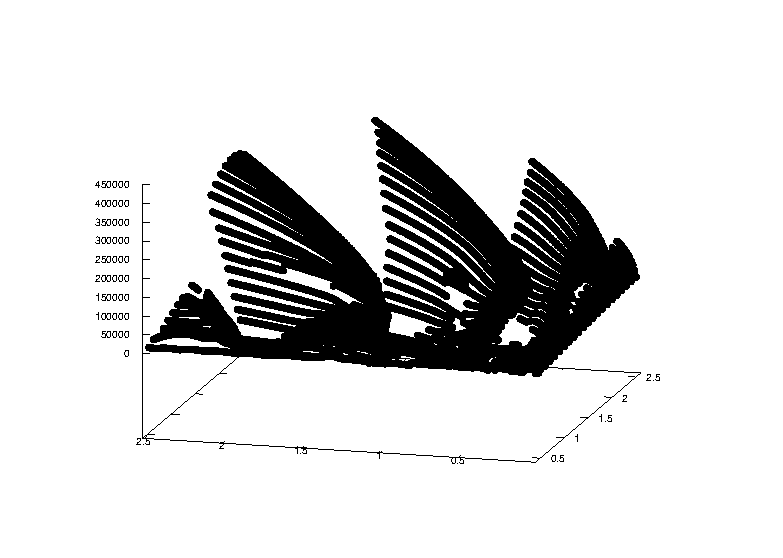
\includegraphics[width=\linewidth,angle=0]{pictures/gnuplot/3d/Hoehe/production/HoeheKraft.eps}
	\end{center}	
\end{figure}
	
	
 

	%Im zweiten Teil des Hauptteils folgt die Darstellung der eigenen Leistung. Aufbauend auf den im vorigen Kapitel erarbeiteten Grundlagen  wird nun der Lösungsweg aufgezeigt. Dabei wird das prinzipielle Vorgehen zum Erreichen der Zielsetzung unter Einbindung der verwendeten Hilfsmittel (Maschinen, Geräte, Programme etc. inklusive der verwendeten Einstellungen) aufgezeigt. Dabei müssen sämtliche verwendeten Daten ersichtlich sein, sodass es jederzeit möglich ist, die ermittelten Ergebnisse zu reproduzieren. Zum Schluss erfolgt unter Berücksichtigung der Randbedingungen eine kritische Analyse der Ergebnisse mit möglichen Unsicherheiten und Fehlern. Aus der Diskussion der Ergebnisse (z.B. Vergleich von Messwerten und theoretischen Vorhersagen), wird schließlich der Nutzen erörtert und mögliche weiterführende Fragestellungen werden erarbeitet.